\section{Introduction}
The decade long search of casual variant by genome wide associatio analysis (GWA) hasn't been satisfying. So far GWA hardly find any single nucleotite variant (SNV) with an large enough effect to act as a stand along necessary cause of any complex diseases. Although a large number of statistically significant common variants were indeed identified by GWA, only a moderate fraction of heritability have been explained by the totality of these finding\cite{GWA1, GWA2}. Despite the setback, human genome is still an intriging source of curiosity owning to its intrisic advantages. When viewed as an exposure, genetic polymophisim is consistant throughout an individual's life course and most types of organism, saving the complication of statistical modeling. Also, as one of the fundermental causes of all biological processes, genomic polymophisim as an exposure, is not suseptable to reverse causality that troubles most non-experimantal designs. From a population perspective, the occurance of genetic variation is random, mimicing a random assignment of exposure in an quasi-experiment, which in turn can be exploited to infer non-genetic effect through an intrumental variable approach, embodied by a Mandilian Randomization design\cite{MR1, MR2}. These features keeps genomic analysis a promising tool for weak effect inference in a complex casual netowrk.

The "common variant, common disease (CVCD)" notion led to the GWA era, as its alternative, the "rare variant, common disease (RVCD)" hypothesis states that the "missing heritability" inexplanable by GWA findings could be attributed to unobserved rare variants of moderate to large effect \cite{RVCD1}. In other words, the so called "whole genome" in GWA was not yet up to its name. The Next Generation Sequencing (NGS) projects, growing in both number and scale over the last decade, facilitated the trial of rare variants. However, as the NGS data keep stockpiling, it also poses a number of new methodological challange. For one, the variants in a NGS profile is much more densely located in the genome, than a typical GWA profile typed by microarrays, which poses serious computational and multiple testing issue should the traditional per-variant screening procedures were applied. Also, as expected, most of the newly called rare variants come with minor allele frequencies (MAF) close to 0. As a direct consequence, such lack of heterogeneity in genotype poses a heavy toll on the statistical power for studies of moderate and smaller sample size. In the epidemiology sence, the number of exposed subjects (either cases or controls) is too small to draw any meaningful inference. So far the most widely accpeted solution is signal aggregation, that is, instead of screening the whole profile one variant after another, one first assign the variants to groups accroding to certain criteria, and subsequently all the variants in one group are test as one unit, by aggregating their signal in a certain way. Commanly, the aggregation can be achieved by collapsing the group into a single variable \cite{Burden1}, or by jointly testing all the variants together \cite{HWU, SKT}. Signal aggregation could be post-screening as well, done by first perform a traditional per-variant GWA screening, then the test statistics (e.g. odds ratio) or its derivation (e.g. the p-values) of a group are combined into a single statistics \cite{Dai:2015, plink1}. Through grouping and aggregation, the number of hypothesis testing reduces to the number of groups, and the heterogeniety of genotype is enchanced to the probability of any variation of the group member. A difficulty comes along with the approach however, is the choice of groupingcriteria. The most popular grouping schemes refer prior knowledge of biological function, resulting in gene or pathway based grouping. Some more debatable schemes rely on the physics of the genome, such as binning the genome by every few kb[?] or by a threshold of linkage disequilibrium (LD) \cite{plink1}. The function based grouping is less subjective and better suited for later interpretation, but for the same reason it is also somewhat a ad-hoc approach, since the ultimate goal of grouping these variants by function, is itself the inference of certain function. Another downside of functional grouping is that it can not exhaustively cover the whole genome, because some variants do not fall into any protein coding gene or known pathway. The physical grouping, on the other hand, could comprehensively cover the entire genome, but is somewhat arbitrary, because the the optimal bin size, LD threshold, and starting position of segmentation, are not pre-known by the investegators. The analytical outcome could also be drastcially different if a different setting was choosen. Aside from signal aggregation, another trend is to form huge, multi-site cohort for large sample such as GIANT and ARIC, or to perform meta-analysis for a large number of published result \cite{META1}, so the sheer number of the observations could overcome the issue of multip testing and low MAF. Now it is not uncommon to apply a brutle per-variant scan for a cohort of more than a thousand subjects. However, the curse of weak effect and low heritability is still lingering, despite frequently reported rare variants reaching statistical significance. The general picture, is still a lack of methodology of moderate prediction power for complexe health outcomes.

The reasons of genetic effects being weak, is in many way like any other fundermantal cause in a casual network, such as social economy status, race/ethnicity and birth place. While being persistant and relatively free from feedback loops, this kind of causes have to reach the final outcomes through a huge "blackbox". As a result, solely altering one dimension of the exposure while leaving the other causes and modifiers untouched won't change the outcome by large. Naturely one would seek amending forces in attempt to unfold the "blackbox", which can be approached from both ends of the casual network. From the downstream end, the bottom-up approach revoles around the central dogma, that is, DNA transcript to mRNA, and mRNA translate to Protein, and thus the profiles of interest are expanded into transcriptome and proteome, respectively. The most prominent practises are expression quantitative trait loci (eQTL)\cite{eQTL1, eQTL2} and gene network analysis. Also from the upstream end, an investegator could collect a variety of strong indicators proximate to the health outcome. Typical examples are conventional biomarkers like inflammatory cytokines, c-reactive protein, serum cholesterol and anti-body titers \cite{cytokine1, CRP1}, and non-conventional biomarkers, such as the neuroimage profiles \cite{VWA1, VWA2, VWA3, VWA4} included by our study. To be noted however, unfolding the "blackbox" is no easy task since any intermidiate factor in the casual network loses the simplicity of a fundermental cause. Namely, an indicators is susceptable to feedback loops and confounders, thus a strong biomarker does not equate to a strong cause, hince the separation of a cause and an indicator. Also, unlike genomic variants, intermidicate indicators are no longer static throughout time and space, for example, the transcriptome of the same subject are quite distinct across different types of cell and life cycle. As an matter of fact, eQTL and gene network analysis are largely seen with, and mostly limited to cancer researches. The downstream strong biomarkers are usually considered as the golden standard of diagnose and confirmation, but are arely suitable for long term risk prediction. A difficulty this work trying to address is the joint analysis of both fundermental casuse and intermidiate factors, either from upstream or downstream. Traditional epidemiology relies on regression to tease apart the direct effect of the fundermental cause and the effect mediated throught the intermidiate factors. This is not suitable when the potential causes in question are groups of tens of hundrends genomic variants, and more ever, when the proximate indicators, in our case, the neuroimage profiles, have even higher dimensionality than an average genomic testing unit.

As mentaioned above, alongsided with the NGS data, the neuroimaging profiles have been incroperated into the statistical models for the added oppertunity to detect associations, and are applied with procedured similar to those designed for genomic analysis. The strength of association between neuroimaging profile and neurological disorder are much higher than from the genome to the same disease \textit{per se} since, the deteriation of cortial surface and subcortical tissue is a proximite event to the final outcome in CNS. Similar to GWA, one could also define a image variant for as the target of statistical inference, which is usually an atomic image unit. For the structure MRI, a variant usually takes the form of a cubic voxel in the 3D volumn spanned by an array of slices [a picture?], which is also an 3D analogy of a square pixel in a 2D plane. The value of voxel taken from the intensity of MRI image, that is, the darkest one has a value of 0, the brightest one is 1. For our study though, the neuroimg profile are not the original MRI and its voxels, but instead we use the 3D cortical surface reconstructed from the structure MRI, performed with the \FS image analysis suite, which is documented and freely available for download online (\url{http://surfer.nmr.mgh.harvard.edu}) \cite{FS:Intro}. Every subject has two cortical surfaces reconstructed, corresponding to the left and right hemispheres, each cortical surface is spanned by 163842 connected vertices, each of which is teated as a variant. The value of a variant(vertex) is no longer the MRI scan brightness, but the gray matter thickness \cite{FS:Tck1, FS:Tck2}, white matter area, gray matter volumn, located around the close proximity of that variant, which is calculated by \FS during the cortical surface reconstruction. The neuroimaging profile, either the brightness of the voxels or the genometry of the vertices, do not suffer the issue of poor signal like the rare genomic variant does, because the values of either type of image units are continuous. Therefore, much like GWA, a per-variant screening can be applied to neuroimage profiles to search for signifiant loci. For analysis using the brightness of voxels from the original MRI slices, this is called voxel-wise analysis (VWA) \cite{VWA1, VWA2, VWA3, VWA4}. As for vertices in the reconstructed surface, \FS comes with its own surface analysis tool which is essentially applying generalized mixed linear regression for each vertex \cite{FS:Anl1, FS:Anl2}, the small area around each vertex is then color coated with the cooresponding $-\log{P}$. A clinical association between neuroanatomical region of interest (ROI) and the health outcome is readly checked by comparing the color pattern of that ROI (Figure \ref{fig:FS1}). In such sense, the \FS surface analysis tool can be called vertex-wise analysis, also abbrevated to VWA. However, the \FS tool is not meat for cohort analysis involving hundreads to thousands participants, because the investigation of color coated surface has to be done by human labor. 
\begin{figure}[h]
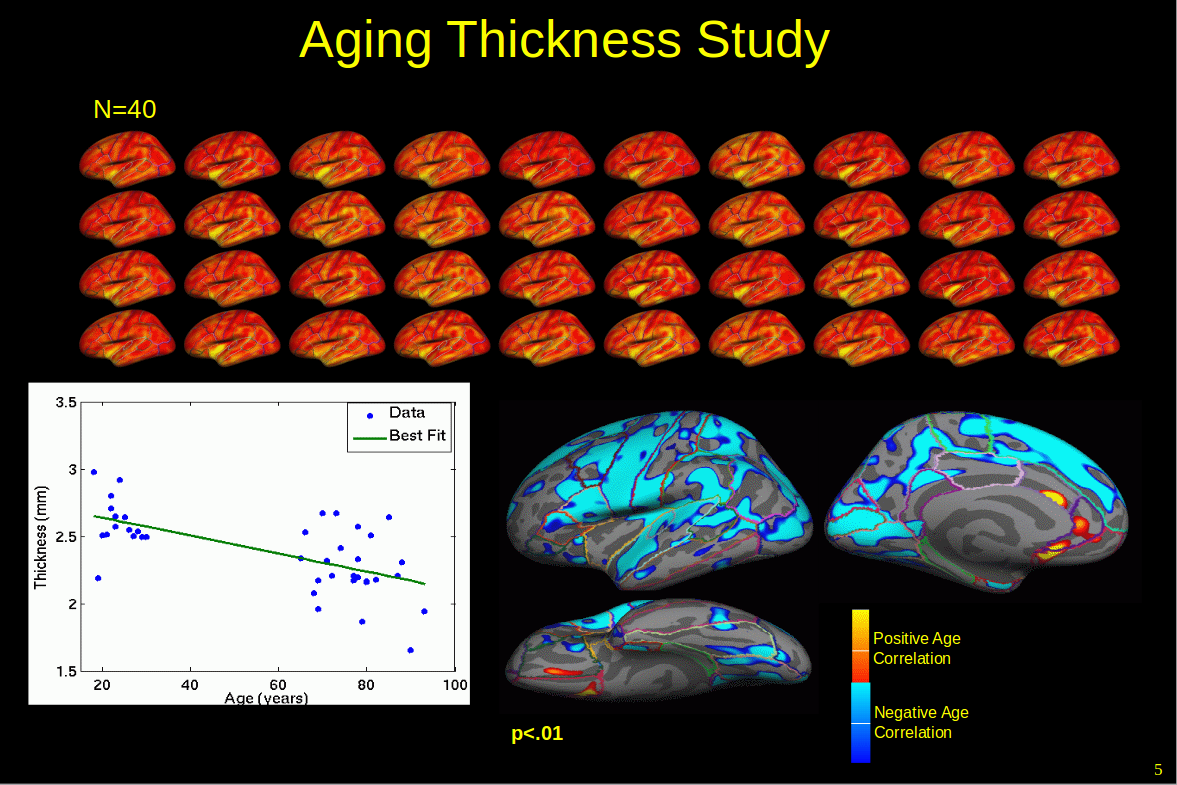
\includegraphics[width=\textwidth]{FS_GLM}
\caption[\FS's Vertex-Wise Analysis]{\FS's Vertex-Wise Analysis}
\label{fig:FS1}
\textbf{top:} 40 sample cortical surfaces color coated by gray matter thickness;
\textsf{bottom left:} fitted $thickness - age$ slop at one of the 327684 vertices;
\textsf{bottom right:} cortical surface color coated by $-log{P}$ of the $thickness - age$ slop at each vertex.
\end{figure}
Recognizing that the closely located variants are clearly highly correlated, the grouping and aggregation accepted by genomic analysis can also be used on image profiles to enhance statistical power[Zhu et. al.].
Before the signal aggregation of a testing unit however, a number of procedures could be applied to the unit to enhance statistical power, which usually involves dimension reduction and noise supression. For genomic profiles, a growing trend is to treat it as a discrate sample drawn from a smooth function [Olga V.]. With a well-balanced emphasize on smoothness and goodness of fit, a small expense of profile accuray can reduce the mean differences among the cases as well as among the controls while enlarging the difference between the two group, achieving higher power. Similar priciple can be applied to any type of high dimensional testing unit, as long as we believe the within group difference are most likely contrubited by noises unexplainable with the case/control membership, thus grinding them away with a smoother helps distinguishing the profile of a case from that of a control. A technic commonly adopted by neuroimaging analysis is to burn away trivial details with a gaussian filter while retaining major features by restricting the size of the filter\cite{VWA1, VWA2, VWA3, VWA4}. In this work however, we construct a stacked autoencoder (SA) for each cortical surface testing unit. Unlike the Gaussian filter who uniformly remove a certain level of detail from the image, an SA is actively looking for meaningful high order features and droping trivias.

We are now seeing an increasingly denser genomic profile with large number of rare variants, and the oppertunity to incroporate high dimensional profiles other than genomics. We propose a similarity based U statistics for the association analysis involving more than one high dimensional profiles; we would also try to tackle the dimensionality and low power issue with signal aggregation, and perticularly to the medical image profiles, we will construct an stacked autoencoder to extract major features of lower dimensionality, and lower noise/signal ratio.